\documentclass{HHUBachelorThesis}

\usepackage{caption}
\usepackage{multirow}

\studentnumber{201002xxxx}
\grade{2020 级}

\title{植物对泥沙沉降规律的影响研究}

% 凑齐 10em
\major{\hspace{10em}}
\name{\hspace{10em}}
\advisor{\hspace{10em}}
\reviewer{\hspace{10em}}

\year = 2024
\month = 6

\titleen{Writing the title of the paper in English here}

\collegeen{XXX XXX}
\subjecten{XXX XXX}
\nameen{X X X}
\advisoren{XXX Professor}

\abstractzh{由于泥沙与水流的相互作用,使得河流发生演变,因此泥沙特性与水流特性均是河流动力学的重要研究课题。当水流中含有植物时,水流的紊动特性会发生明显的改变,从而引起泥沙的一些特性如沉速发生改变。本文以实验为基础,结合理论分析,研究了在静水条件下刚性植物对泥沙沉速的影响,同时在水槽中通过改变流量来研究在恒定均匀流条件下非淹没植物对泥沙沉降轨迹的影响,得到如下主要结论:}
\keywordszh{关键词 1;关键词 2;关键词 3}
\abstracten{Fluvial river processes evolve over time in response to the constant interaction between sediment and the water column. If vegetation is present within the water column, the change in turbulence characteristics will impact the movement of sediment, in particular the settling velocity. In this paper, the influence of vegetation on the settling velocities of sediment particles is studied experimentally. The non-submerged vegetation friction factor in steady uniform flow is considered by under different flumedischarge quantities. The main outcomes can be summarized as follows:}
\keywordsen{sediment;rigid vegetation;settling velocity;turbulence characterize}

\begin{document}

\ChineseCover
\EnglishCover
\AcademicStatement
\AbstractzhPage
\AbstractenPage
\ToCPage

\section{绪论}

\subsection{问题的提出及研究意义}

泥沙在自然界中的河流中普遍存在着,泥沙含量的不同影响着河流流态,加上各种泥沙特性不同,使得河流泥沙问题更加复杂多变。\cite{钱宁1983} 如广泛分布在黄河流域一带的黄土地质均匀,其粉砂含量占 $60\%\sim70\%$,缺乏团粒结构,粒间的固结主要依靠硫酸钙质,这种硫酸钙质遇水极易溶解流失,加上黄土孔隙率极高,抗蚀能力很差。

\subsubsection{问题提出}

近年来,随着环境的日益恶化,人们对生态日益重视,含有植物的水流问题也已经成为河流动力学研究中的热点之一。\cite{唐洪武2007} 直观的了解,河渠水流中的植物不仅减少了过水面积,加大了河渠地面的粗糙程度,降低了河渠的行洪能力,加大了两岸的洪灾威胁。\cite{kouwen1969,Gourlay1970}

\subsubsection{研究意义}
\subsection{泥沙沉速的研究概述}
\subsubsection{泥沙沉速的影响因素}
\subsubsection{泥沙沉降阻力系数}
\subsubsection{泥沙沉速公式}
\subsubsection{动水中泥沙沉降的计算方法}
\subsection{植物对泥沙沉降的影响概述}
\subsubsection{植物对静水中泥沙沉速的影响}
\subsubsection{植物对明渠水流中泥沙沉降的影响}

\clearpage

公式、图文示例:

(1)公式示例:单颗粒球体在无限水体中等速下沉时,其沉速机理可看作对称绕流阻力与颗粒有效重力相平衡,即 \begin{equation}
    (\gamma_s - \gamma) \cdot \pi \frac{D^3}{6} = C_D \pi \gamma \cdot \frac{\omega^2}{2 g} \cdot \frac{D^2}{4}
\end{equation}

Stokes 曾以粘滞性流体的一般性的运动方程式作基础,忽略惯性项的条件下推导出滞留区的阻力系数为 \begin{equation}
    C_D = 24 / \mathrm{Red}
\end{equation}

(2)表示例:\begin{table}[h]
    \zihao{5}
    \centering
    \caption{光滑明渠水流实验水力条件}
    \begin{tabular}{|c|c|c|c|c|c|}
        \hline
        \multirow{2}{*}{\bfseries \songti \begin{tabular}[c]{@{}c@{}}实验\\ 编码\end{tabular}} & \textbf{H} & \textbf{G} & \textbf{J}       & \textbf{B} & $U_*$  \\ \cline{2-6}
                                                                                           & cm         & L/s        & \textperthousand & cm         & cm/s   \\ \hline
        w1                                                                                 & $18$       & $7.56$     & $0.02$           & $42$       & $0.19$ \\ \hline
        w2                                                                                 & $18$       & $11.34$    & $0.07$           & $42$       & $0.68$ \\ \hline
        w3                                                                                 & $18$       & $15.12$    & $0.13$           & $42$       & $1.27$ \\ \hline
        w4                                                                                 & $18$       & $18.9$     & $0.21$           & $42$       & $2.05$ \\ \hline
        w5                                                                                 & $18$       & $22.68$    & $0.28$           & $42$       & $2.73$ \\ \hline
    \end{tabular}
    \caption*{其中:$U_*$ 为摩阻流速,$U_* = \sqrt{J R g}$(其中 $R$ 为水力半径);$J$ 为水力坡降,$B$ 为水槽宽度,$H$ 为水深。}
\end{table}

(3)图示例:\begin{figure}[h]
    \centering
    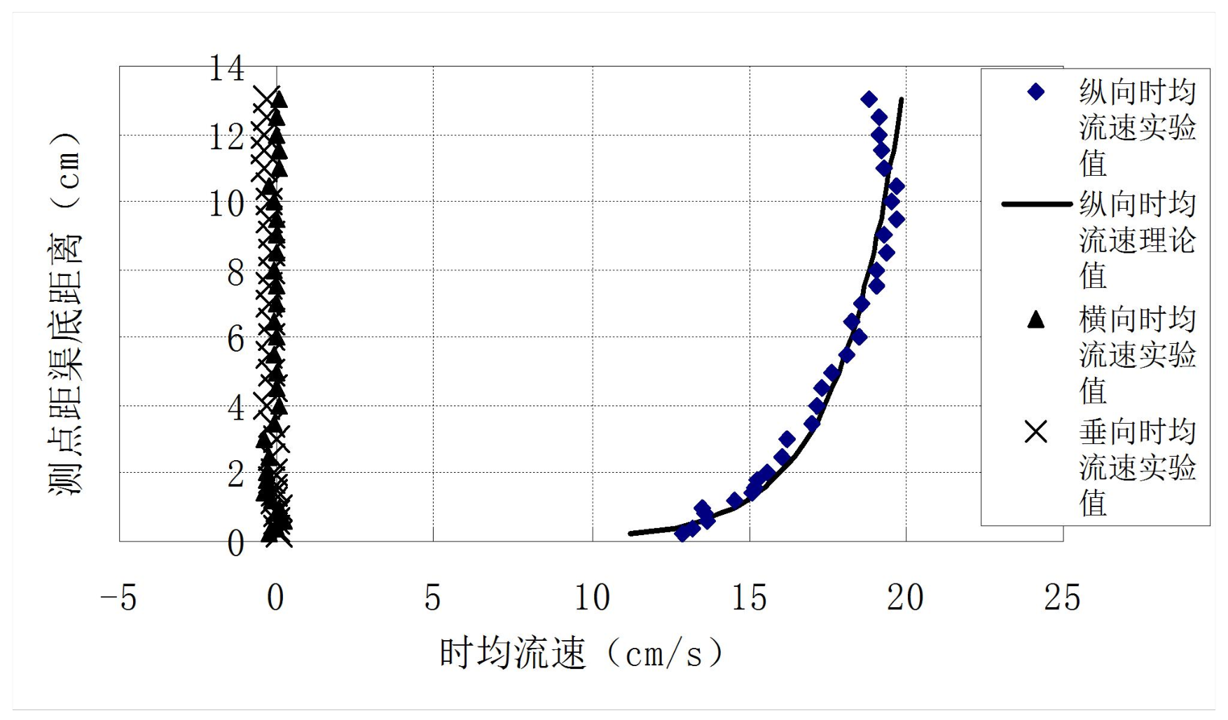
\includegraphics[width=\textwidth]{./media/HHUBachelorThesis.png}
    \caption{清水明渠水流下 w2 工况下的三维时均流速图}
\end{figure}

\clearpage\thispagestyle{empty}
\bibliography{HHUBachelorThesis}\phantomsection\addcontentsline{toc}{section}{参考文献}
\end{document}
